% These are the lecture notes for my CSC1101 course Fall 2016
% at CityTech. They are based largely on How To Think Like A
% Computer Scientist. See last slide for reference information.

% Feel free to edit these slides and use them for your own courses.
% HOWEVER DO NOT REMOVE THESE LINES!
% Email me at: awood [at] citytech.cuny.edu
% or at: awood [at] gradcenter.cuny.edu



\documentclass{beamer}

\usepackage{tikz}
\usetikzlibrary{calc}

\usepackage{forest}
\usepackage{verbatim}
\usepackage{alltt}

\setbeamertemplate{footline}[frame number]
\setbeamertemplate{navigation symbols}{} 

\newtheorem{thm}{Theorem}[section]
\newtheorem{lem}{Lemma}
\newtheorem{cl}{Claim}
\newtheorem{cor}{Corollary}[section]
\newtheorem{conj}{Conjecture}
\newtheorem{quest}{Question}
\newtheorem{defn}{Definition}[section]
\newtheorem{obs}{Observation}[section]
\newtheorem{exam}{Example}

\mode<presentation>
{
%  \usetheme{default}
  \setbeamercovered{invisible}
}


\usepackage[english]{babel}
\usepackage[latin1]{inputenc}
\usepackage{times}
\usepackage[T1]{fontenc}
\usepackage{stmaryrd}

%\usetheme{default}
%\usetheme{AnnArbor}
%\usetheme{Antibes}
%\usetheme{Bergen}
%\usetheme{Berkeley}
%\usetheme{Berlin}
%\usetheme{Boadilla}
%\usetheme{CambridgeUS}
%\usetheme{Copenhagen}
%\usetheme{Darmstadt}
%\usetheme{Dresden}
%\usetheme{Frankfurt}
%\usetheme{Goettingen}
%\usetheme{Hannover}
%\usetheme{Ilmenau}
%\usetheme{JuanLesPins}
%\usetheme{Luebeck}
%\usetheme{Madrid}
%\usetheme{Malmoe}
%\usetheme{Marburg}
%\usetheme{Montpellier}
%\usetheme{PaloAlto}
%\usetheme{Pittsburgh}
%\usetheme{Rochester}
\usetheme{Singapore}
%\usetheme{Szeged}
%\usetheme{Warsaw}

%\usecolortheme{default}
%\usecolortheme{albatross}
\usecolortheme{beaver}
%\usecolortheme{beetle}
%\usecolortheme{crane}
%\usecolortheme{dolphin}
%\usecolortheme{dove} % grey, white, yellow
%\usecolortheme{fly} %grey, yellow
%\usecolortheme{lily} %white, yellow, blue
%\usecolortheme{orchid}
%\usecolortheme{rose}
%\usecolortheme{seagull}
%\usecolortheme{seahorse}
%\usecolortheme{whale}
%\usecolortheme{wolverine}


\title[Conditional Execution]{Python 2.7: Conditional Execution}
\author
{Lecture notes of Alexander Wood \\ \scriptsize \href{mailto:awood@citytech.cuny.edu}{awood@citytech.cuny.edu}}
\institute[CityTech]{New York City College of Technology }  

\date{}

\begin{document}

%%%%
\begin{frame}
\titlepage
\end{frame}

\section{Code Structures Review}

%%%%
\begin{frame}[fragile]
\frametitle{Code Structures}

\begin{itemize}
\item Many languages use curly braces or characters such as \verb|begin| and \verb|end| to designate sections of code
\item Recall that Python uses \textbf{indentation to define a program's structure}
\item You can use any indentation you want but Python expects you to be consistent. The recommended style is four spaces.
\end{itemize}
\end{frame}

%%%%
\begin{frame}
\frametitle{Code Structures: Comments}

Write \textbf{comments}, pieces of text that the program interpreter ignores, using the hashtag. 
\begin{figure}
\centering
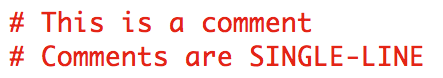
\includegraphics[scale=.5]{IMG/1.png}
\end{figure}
However, you can write multiline quotes in your code and then not print them to write multiple lines of unread text.
\begin{figure}
\centering
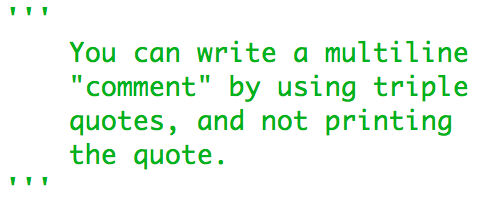
\includegraphics[scale=.4]{IMG/2.png}
\end{figure}
A hashtag inside of a print statement is NOT a comment.
\begin{figure}
\centering
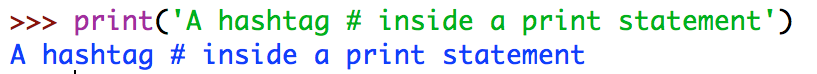
\includegraphics[scale=.5]{IMG/3.png}
\end{figure}
\end{frame}







\section{if Statement}

%%%%
\begin{frame}
\frametitle{Decision Structures}

Code is executed sequentially, or line-by-line.
We can control which lines of code are executed with \textbf{decision structures}.
\end{frame}

%%%%
\begin{frame}[fragile]
\frametitle{The if Statement}

The \verb|if| statement is the first example of a decision structure we shall see. It has the following syntax:
\begin{alltt}
if condition:
    statement
    statement
    statement
\end{alltt}
\end{frame}

%%%%
\begin{frame}[fragile]
\frametitle{The if statement}

The \verb|if| statement checks a condition is true. If the condition is true, the statements inside of the if condition are executed.

\begin{figure}
\centering
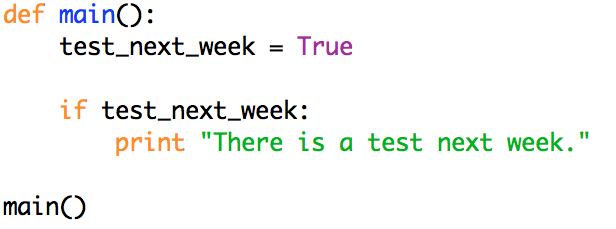
\includegraphics[scale=0.8]{IMG/if.png}
\end{figure}
\end{frame}

%%%%
\begin{frame}
\frametitle{The pass statement}

There is no limit on the number of statements that can be in an if statement, but there has to be at least one. You can use the \textbf{pass} statement as a placeholder for code you will fill in later.

\begin{figure}
\centering
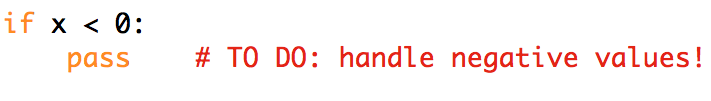
\includegraphics[scale=0.8]{IMG/9.png}
\end{figure}
\end{frame}

%%%%
\begin{frame}
\frametitle{Example Problem}

In class, we translate the flowchart from Quiz 1 into a Python program.
\end{frame}


%%%%
\begin{frame}
\frametitle{Example: If}

Write a program which asks a user for their grade. If it is above or equal to $70$, tell them they passed.

\end{frame}


%%%%
\begin{frame}
\frametitle{Solution}

\begin{figure}
\centering
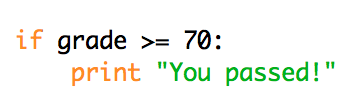
\includegraphics[scale=0.8]{IMG/if_grade.png}
\end{figure}
\end{frame}








\section{If-Else}

%%%%
\begin{frame}[fragile]
\frametitle{if-else}

It is also possible to specify what will happen if the if condition is not satisfied, using \textbf{else}. The syntax is as follows:
\begin{alltt}
if condition:
    statement
    
else:
    statement
\end{alltt}
\end{frame}

%%%%
\begin{frame}[fragile]
\frametitle{if-else}

If \verb|test_next_week| is \emph{not} true, the \verb|else| condition is executed.

\begin{figure}
\centering
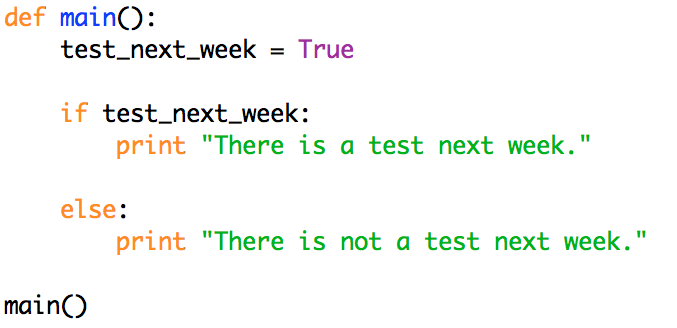
\includegraphics[scale=0.8]{IMG/5.png}
\end{figure}
\end{frame}

%%%%
\begin{frame}
\frametitle{Exercise: If-Else}

Write a program which asks the user for their grade. If their grade is greater than or equal to $70$, tell them they passed. Otherwise, tell them they failed.
\end{frame}

%%%%
\begin{frame}
\frametitle{Solution!}

\begin{figure}
\centering
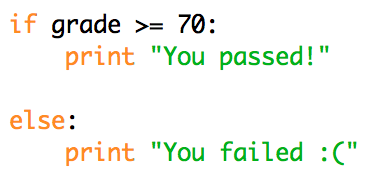
\includegraphics[scale=0.8]{IMG/ifelse_grades.png}
\end{figure}
\end{frame}








\section{Nested Decision}

%%%%
\begin{frame}[fragile]
\frametitle{Nested Decision}

We may also have \emph{nested decision structures}, or decision structures inside of decision structures.

\begin{figure}
\centering
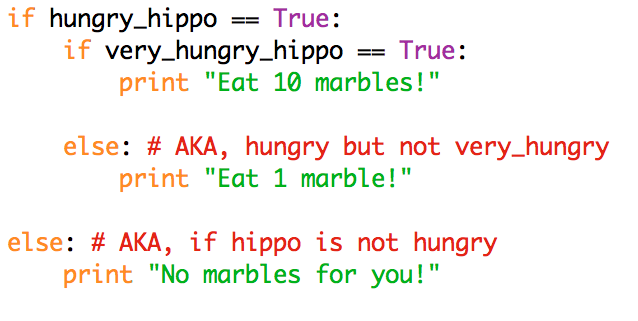
\includegraphics[scale=0.8]{IMG/hippo.png}
\end{figure}
\end{frame}

%%%%
\begin{frame}
\frametitle{Nested Decision}

They may be nested arbitrarily deep.

\begin{figure}
\centering
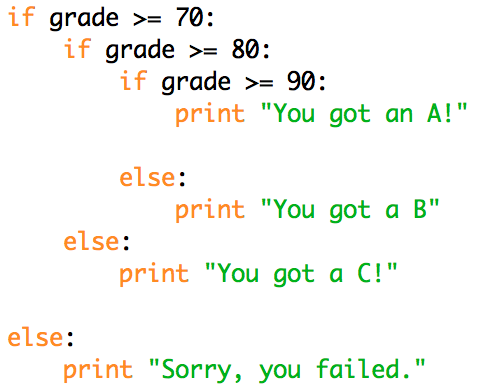
\includegraphics[scale=0.8]{IMG/nested_grade.png}
\end{figure}
\end{frame}






\section{if-elif-else}

%%%%
\begin{frame}[fragile]
\frametitle{Nested Decision vs. if-elif-else}

The previous slide's example runs correctly, but looks messy. We can rewrite nested decision structures using \verb|elif|, which stands for ``else, if."
\end{frame}


%%%%
\begin{frame}[fragile]
\frametitle{Nested decision with if-elif-else}

\verb|elif| allows us to consider multiple possibilities, and has syntax as follows:

\begin{alltt}
if condition:
    statement
    
elif condition:
    statement
    
else:
    statement
\end{alltt}
\end{frame}


%%%%
\begin{frame}[fragile]
\frametitle{Example: if-elif-else} 

Exercise: Rewrite the nested grades example using \verb|elif| (with no nesting.)
\end{frame}


%%%%
\begin{frame}
\frametitle{Solution!}

\begin{figure}
\centering
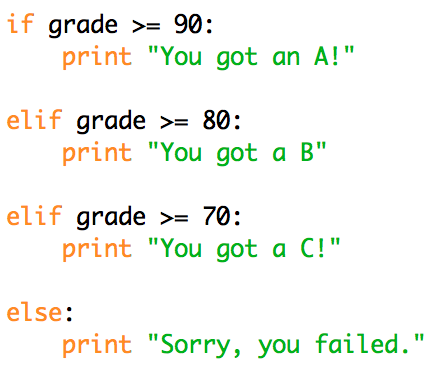
\includegraphics[scale=0.8]{IMG/elif_grade.png}
\end{figure}
\end{frame}


%%%%
\begin{frame}[fragile]
\frametitle{Why elif?}

What if we wrote the previous example using only \verb|if|, and no \verb|elif| statements?

\begin{figure}[h]
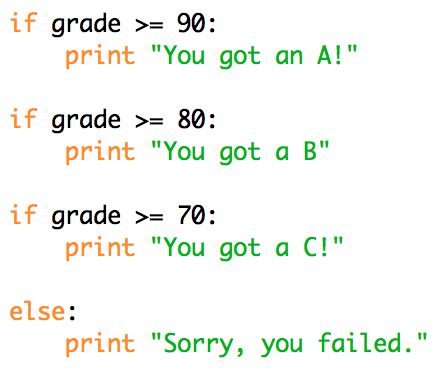
\includegraphics[width=.48\linewidth]{IMG/boo.png}
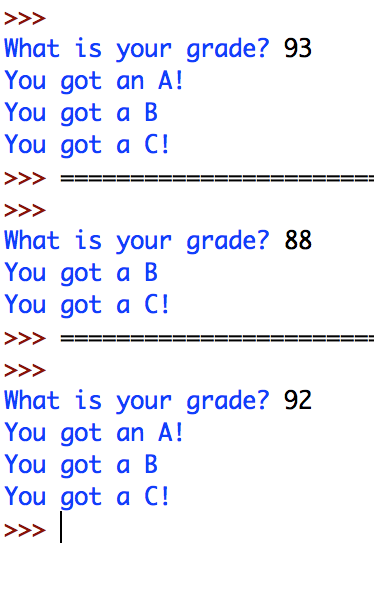
\includegraphics[width=.3\linewidth]{IMG/output.png}
\caption{Output with if statements for various grades}
\end{figure}
\end{frame}


%%%%
\begin{frame}[fragile]
\frametitle{Why elif?}

The \verb|elif| statement can be interpreted as ``otherwise, if..." It forces the cases to be \emph{mutually exclusive.} The grades example does not work without \verb|elif| because the conditions are not mutually exclusive. However, using \verb|elif| forces the cases to be mutually exclusive. 
\end{frame}

%%%%
\begin{frame}[fragile]
\frametitle{Why elif?}

\begin{figure}[h]
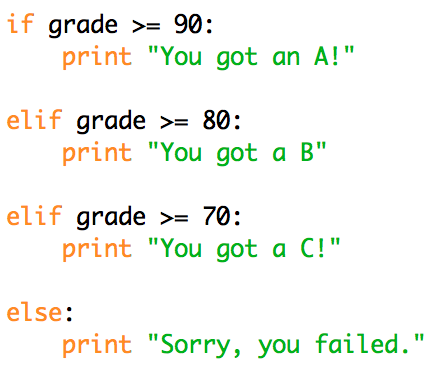
\includegraphics[width=.48\linewidth]{IMG/elif_grade.png}
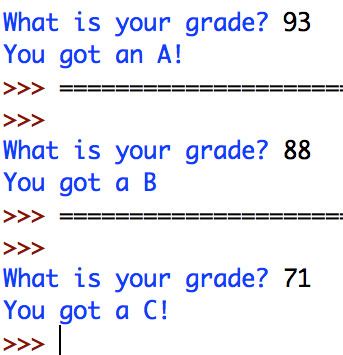
\includegraphics[width=.4\linewidth]{IMG/niceoutput.png}
\caption{Output with elif for various grades}
\end{figure}
\end{frame}


%%%%
\begin{frame}
\frametitle{Cases which shouldn't be mutually exclusive}

Decide if you want your cases to be mutually exclusive or not before deciding upon a decision structure.
\end{frame}

%%%%
\begin{frame}[fragile]
\frametitle{Mutually exclusive?}

Consider the following example, which tests whether a value is positive and whether it is even.
\begin{figure}
\centering
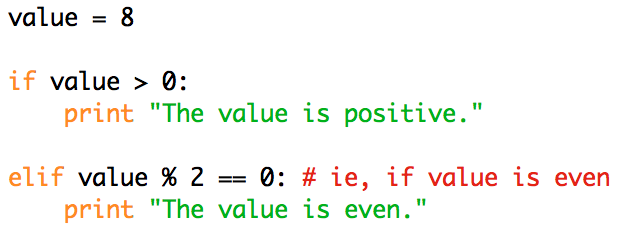
\includegraphics[scale=0.6]{IMG/ex.png}
\end{figure}

The value $8$ is both positive and even. However when we run the program, the output is:
\begin{figure}
\centering
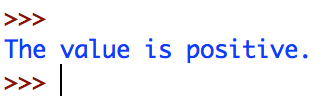
\includegraphics[scale=0.6]{IMG/ex_out.png}
\end{figure}
\end{frame}

%%%%
\begin{frame}[fragile]
\frametitle{Mutually exclusive? No.}

The \verb|elif| structure is for \emph{mutually exclusive} cases, but a number can be \textbf{both} positive and even! Rewrite as follows
\begin{figure}
\centering
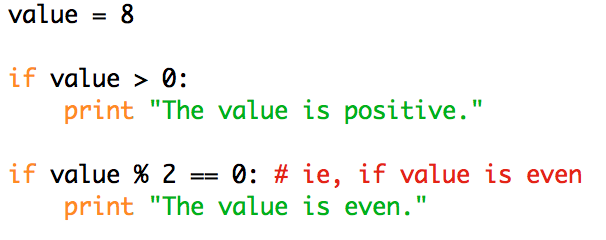
\includegraphics[scale=0.6]{IMG/ex2.png}
\end{figure}
to receive output
\begin{figure}
\centering
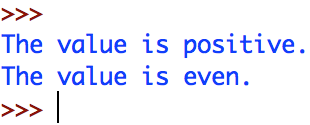
\includegraphics[scale=0.6]{IMG/ex2_out.png}
\end{figure}
\end{frame}


%%%%
\begin{frame}[fragile]
\frametitle{Mix and match!}

We can combine nested decision structures and \verb|elif| to create even more complicated algorithms. The following two algorithms are, in fact, equivalent; one uses \emph{nesting} while the other uses \verb|elif|.


\begin{figure}[h]
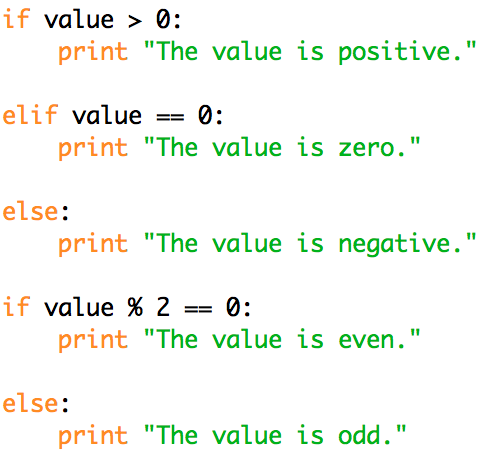
\includegraphics[width=.45\linewidth]{IMG/mixandmatch.png}\hfill
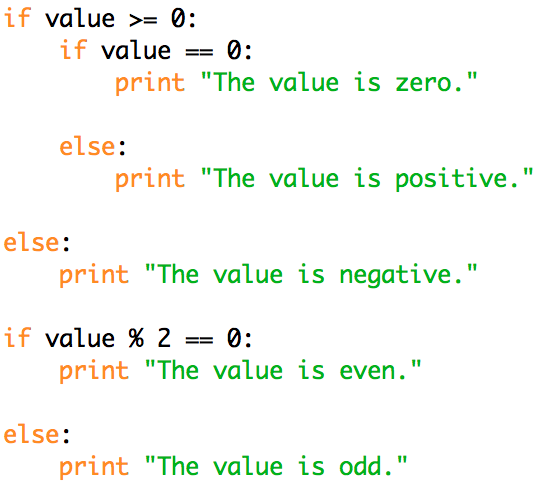
\includegraphics[width=.45\linewidth]{IMG/mixandmatch2.png}
\end{figure}


\end{frame}


%%%%
\begin{frame}[fragile]
\frametitle{Example: Converting from nested to elif}

Convert the following program to \verb|elif| structure; in other words, rewrite it so that there are no nested conditions!
\\
\begin{figure}
\centering
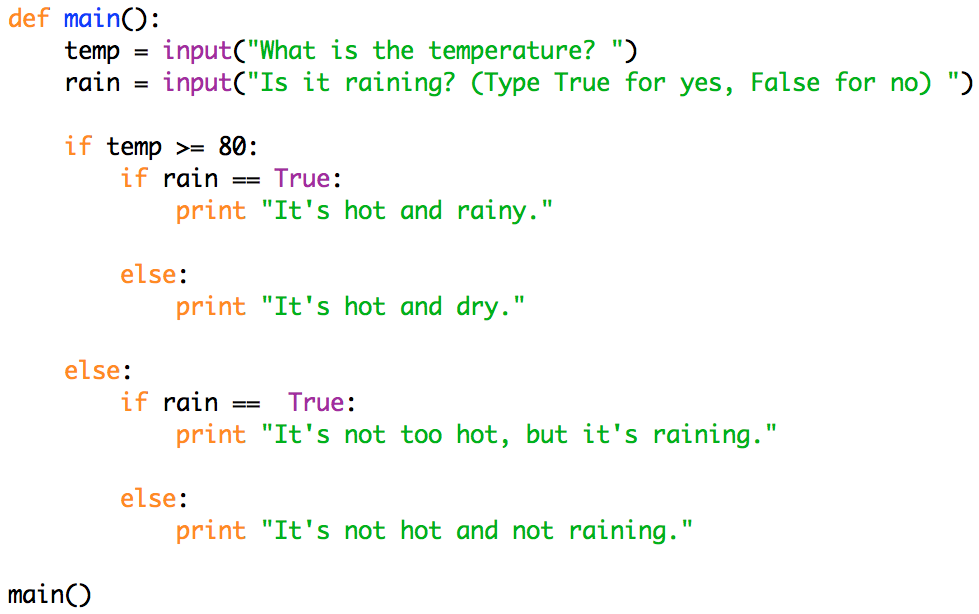
\includegraphics[scale=0.6]{IMG/nested_ex.png}
\end{figure}
\end{frame}


%%%%
\begin{frame}
\frametitle{Solution!}

\begin{figure}
\centering
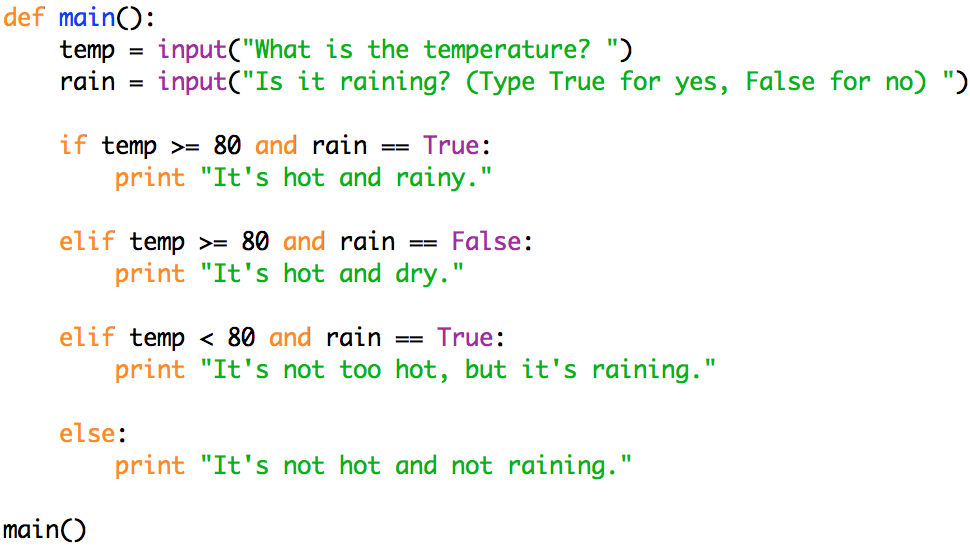
\includegraphics[scale=0.6]{IMG/weather_elif.png}
\end{figure}
\end{frame}

%%%%
\begin{frame}[fragile]
\frametitle{An Observation}

Note that the examples we have used so far have been naive, in that they assume the user inputs their answer as the correct data type, in the correct range. (For instance, if the user set \verb|rain| equal to \verb|7| in the previous example, what would happen?)
\end{frame}

%%%%
\begin{frame}[fragile]
\frametitle{Exercise: Working with the user}

Write a program which asks the user to write a positive integer. If the user writes something which is not a positive number of data type \verb|int|, display the message ``I'm sorry, incorrect input."
\end{frame}

%%%%
\begin{frame}
\frametitle{Solution}


\begin{figure}
\centering
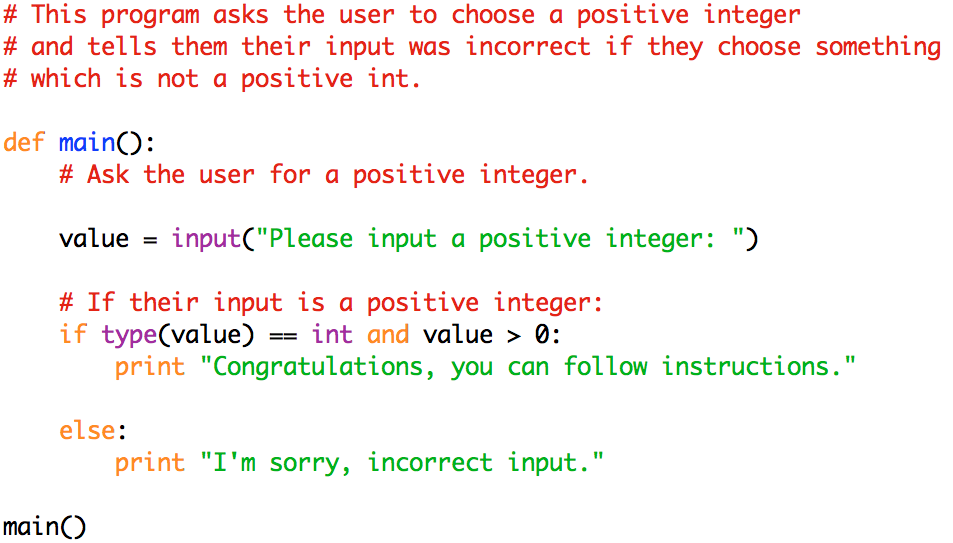
\includegraphics[scale=0.6]{IMG/solution.png}
\end{figure}
\end{frame}


%%%%
\begin{frame}
\frametitle{Further reading}

\begin{itemize}
\item How to think like a computer scientist: Learning with Python, chapter 4
\url{http://www.openbookproject.net/thinkcs/python/english2e/ch04.html}
\end{itemize}
\end{frame}
\end{document}


